%!TEX root = ../Base.tex

\chapter{Experimentos y resultados}\label{ch:chap5}

En los capítulos anteriores se ha descrito los diferentes algoritmos que se utilizarán para realizar la tarea de \sd, y que en esta sección se emplearán de acuerdo al marco experimental que se describe a continuación.

Inicialmete, las pruebas consistieron en usar los algoritmos presentados para selección de modelo usando datos que fueron generados aleatoriamiente a partir de los parámetros de un HMM inicial; para tener una idea general de su desempeño individual.

Para estas primeras pruebas, se simuló una cadena de Márkov oculta con en base en parámetros fijos, con lo que se generó tanto una secuencia de datos observados, como los supuestos datos o variables ocultas que forman la cadena de Márkov. Se utilizó muestreo ancestral para la simulación de estos datos.

Para un caso en específico, se tiene lo siguiente. Realizando la inferencia de parámetros del HMM, se obtienen los siguientes resultados:

El primer algoritmo que se prueba, es el de selección de modelo usando un BIC.

Como ya se comentó, se usará una variante de BIC en donde se incorpora un término de regularización $\lambda$ para que correspondan en órdenes de magnitud tanto la log-verosimilitud del modelo encontrado como su penalización respectiva.

El problema inmediato que se presenta, es cómo realizar la selección del parámetro de regularización $\lambda$ que penalice de forma correcta la verosimilitud para los diferentes modelos propuestos. Si $\lambda$ es demasiado pequeño, entonces la penalización realmente no tendrá efecto y dado el sobreajuste que se presenta al usar modelos más complejos, se preferirán siempre los modelos con más parámetros. Por otro lado, si al escoger $\lambda$ se da demasiado peso al término de penalización, entonces siempre se preferirán los modelos más sencillos.

Para encontrar el valor de $\lambda$ adecuado, se puede entonces formar una superficie con las diferentes curvas de selección BIC de acuerdo a cómo varía $\lambda$, e inspeccionar esta duperficie para encontrar una región de confianza en la que el valor de $\lambda$ es el adecuado.

Por otro lado, para la segunda prueba, se procedió a usar bootstrap con la estadística log-likelihood ratio como ya se describió anteriormente en el \autoref{ch:chap3}, y haciendo la prueba de hipótesis del modelo de $n$ estados contra el de $n+1$ estados.

\section{Experimentos} % (fold)
\label{sec:experimentos}

Para los experimentos realizados, se generaron mediante un sintetizador de voz (también conocido como Text-To-Speech o TTS por sus siglas en inglés) que nos permitió tener un mayor control sobre el contenido como tal de las grabaciones, así como sobre los posibles ruidos o interferencias en las secuencias de audio.

Si bien, para probar el desepeño contra otras propuestas del estado del arte se suelen usar otro tipo de bases de datos, éstas suelen no estar disponibles de forma libre, por lo que preferimos generar nosotros un pequeño dataset con el sintetizador de voz.

Usando dos motores para el sintetizador de voz, uno con voces en inglés y otro con voces en español, se generaron 6 secuencias de audio (3 en cada idioma) cuya duración así como el número de interlocutores que participan varía.

\subsubsection{Prueba 1: Calderon de la Barca} % (fold)
\label{ssub:calderon}

En esta primer secuencia, se tomaron fragmentos de la obra 'La vida es sueño', de Calderón de la Barca, y se utilizaron 3 diferentes voces en español. La secuencia de audio original es de 1:07m.

Para la etapa de agrupación de los vectores MFCC con k-means++ se usaron 160 centros iniciales.

\setlength{\abovecaptionskip}{-10pt plus 0pt minus 0pt}

\begin{figure}[bth]
  \centerline
  {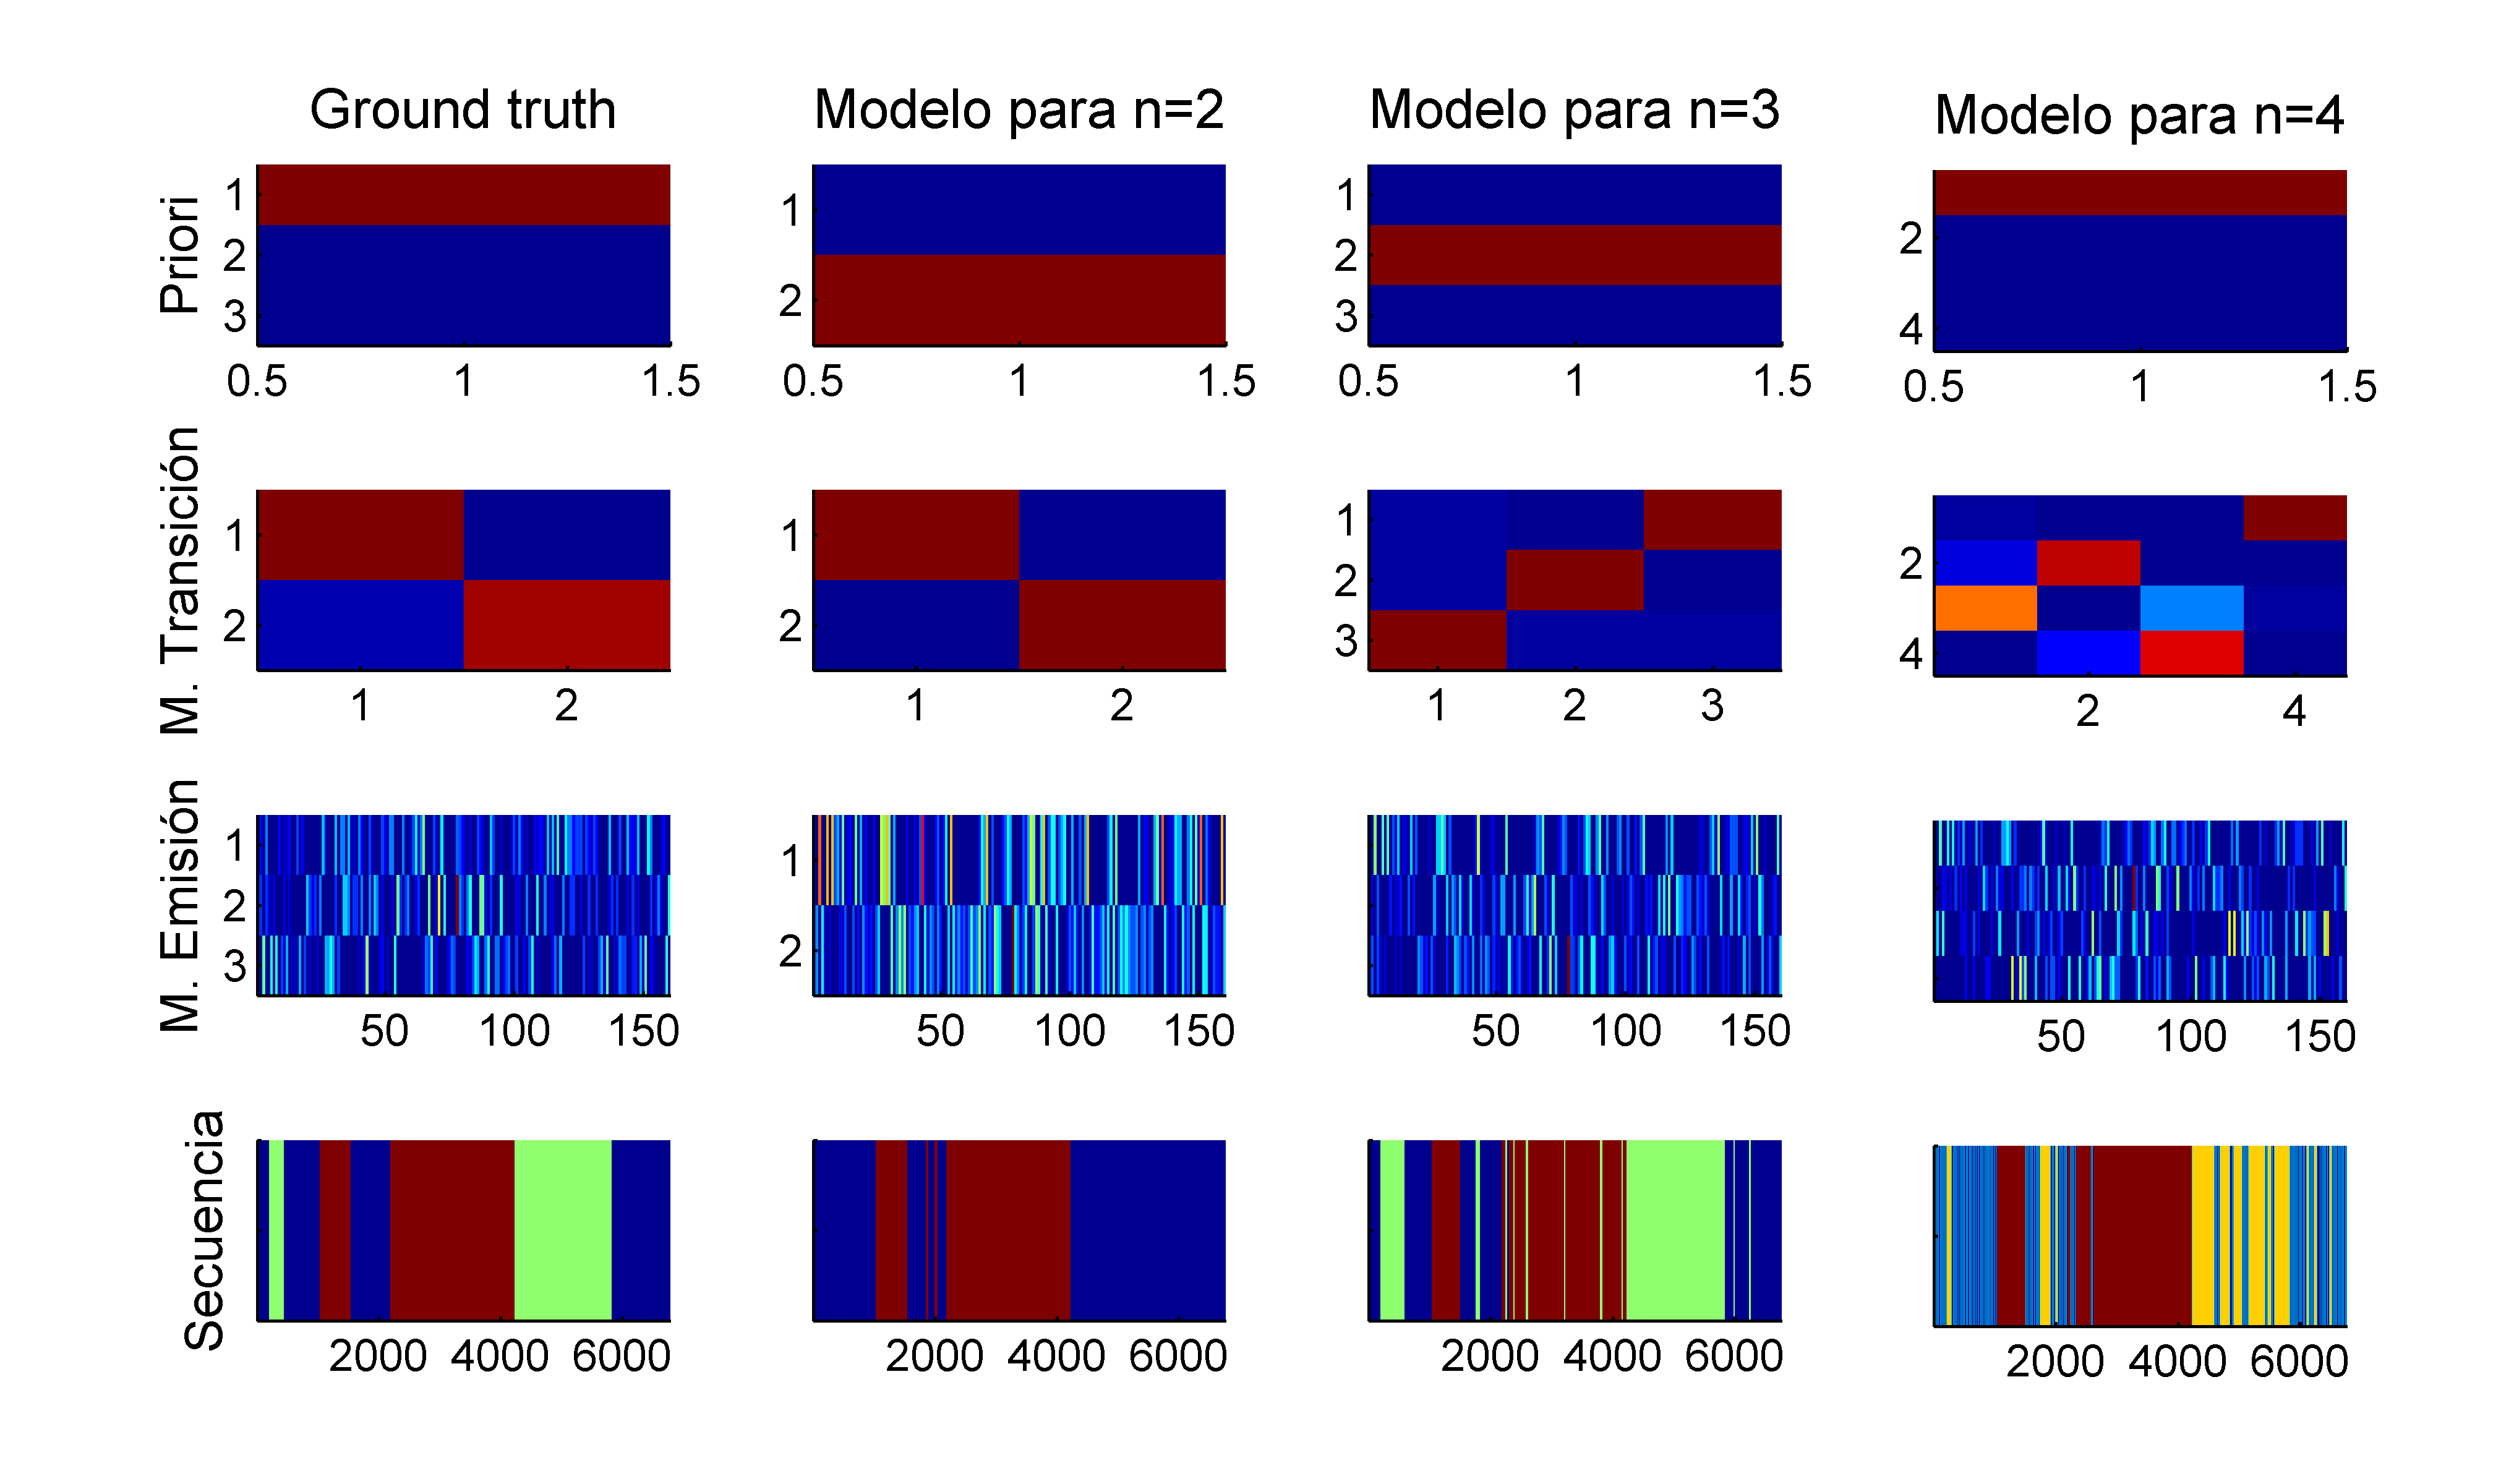
\includegraphics[width=1.1\linewidth]{gfx/chap6/cald1}} \quad
  \caption{Parámetros encontrados para Prueba 1.}
  \label{fig:prb1_par}
\end{figure}

En la \autoref{fig:prb1_par} se muestran los parámetros obtenidos para diferentes modelos que se propusieron. Se observa como para el modelo correcto tanto la matriz de emisión así como la secuencia en falso color corresponden con el ground truth.

Más a detalle, en la \autoref{fig:prb1_seq} se observa en azul el orden en el que participan los interlocutores de acuerdo a la secuencia recuperada. En rojo se marcan tanto los falsos positivos como los falsos negativos, de acuerdo al ground truth. Hay que notar que cuando el número de estados para un modelo no es el correcto, entonces inminentemente el número de errores en la secuencia obtenida será mayor, pues al menos todas las intervenciones de un hablante no podrán ser emparejadas o serán asignadas a alguien más.

Se observa también que la mayoría de las veces, en la secuencia recuperada se encuentran algunos brincos entre personas, pero en esencia la estructura y el orden en que hablan los interlocutores es el correcto.

\begin{figure}[h]
  \centerline
  {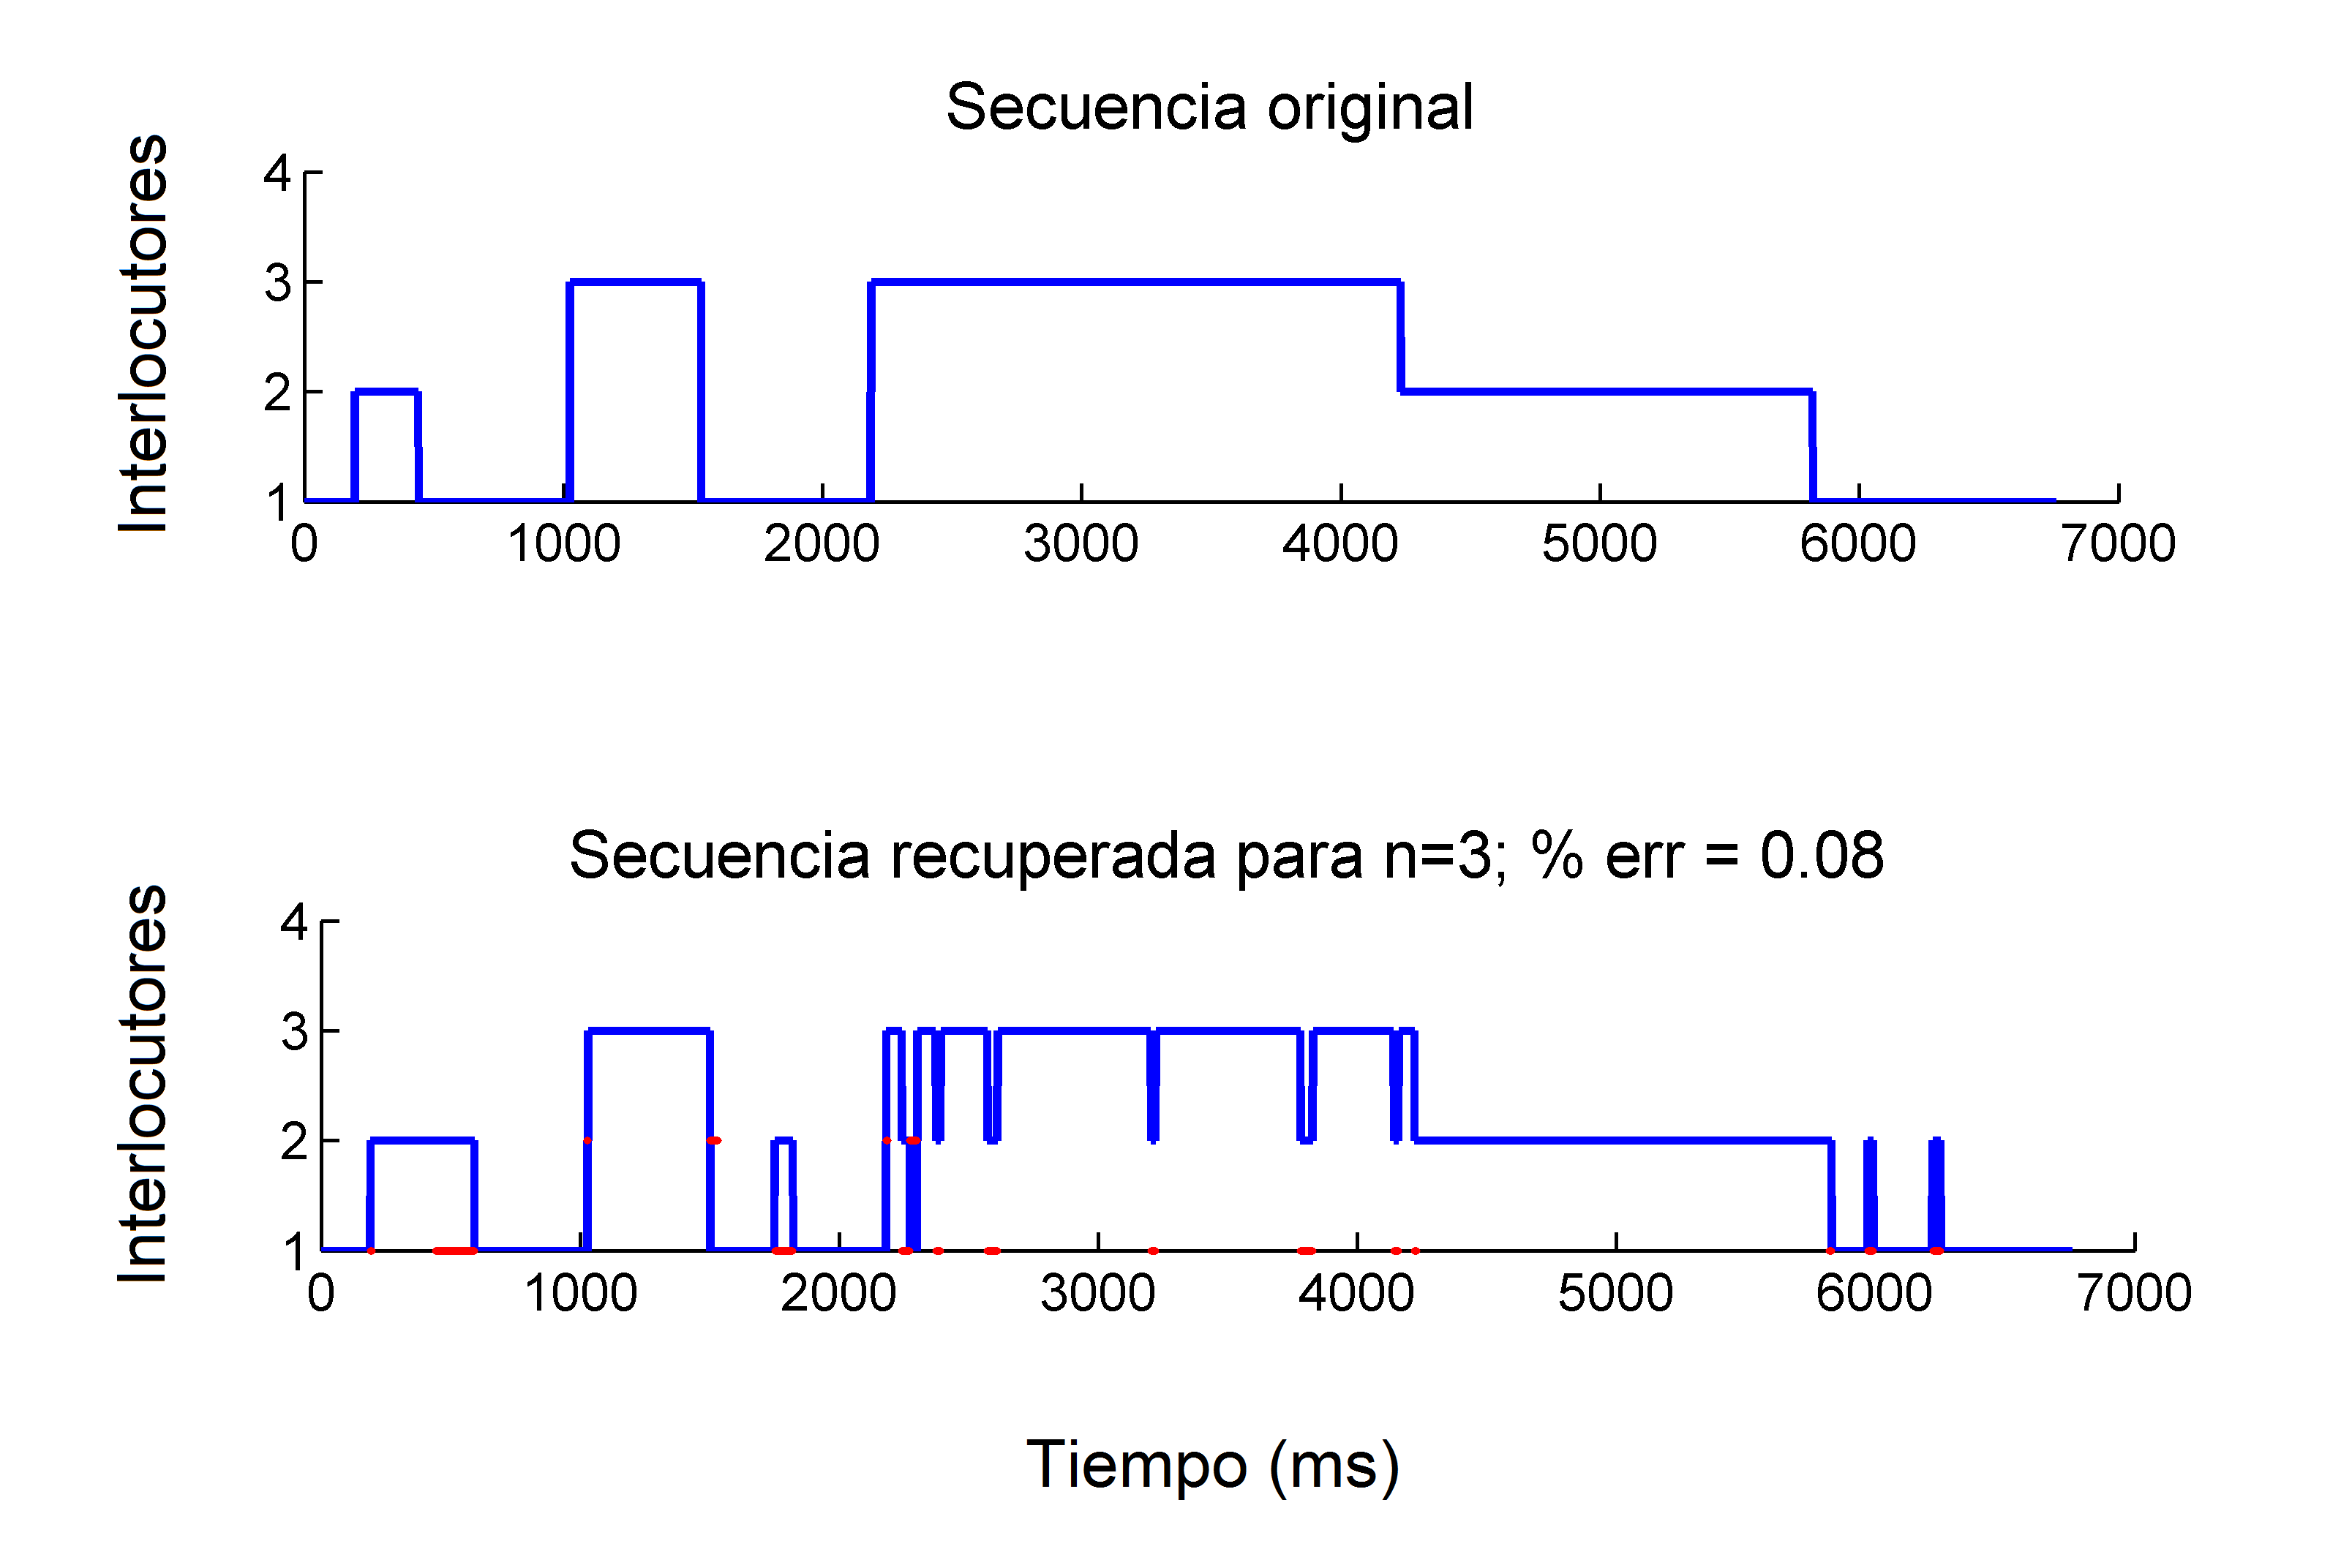
\includegraphics[width=0.8\linewidth]{gfx/chap6/cald1_}} \quad
  \caption{Secuencias encontradas para Prueba 1.}
  \label{fig:prb1_seq}
\end{figure}

Hasta ahora, se han propuesto varios modelos, y si se compara con el ground truth se puede llegar a discriminar cuál es el modelo correcto ya sea por inspección visual o comparando el error absoluto.

\begin{figure}[bth]
  \centerline  
  {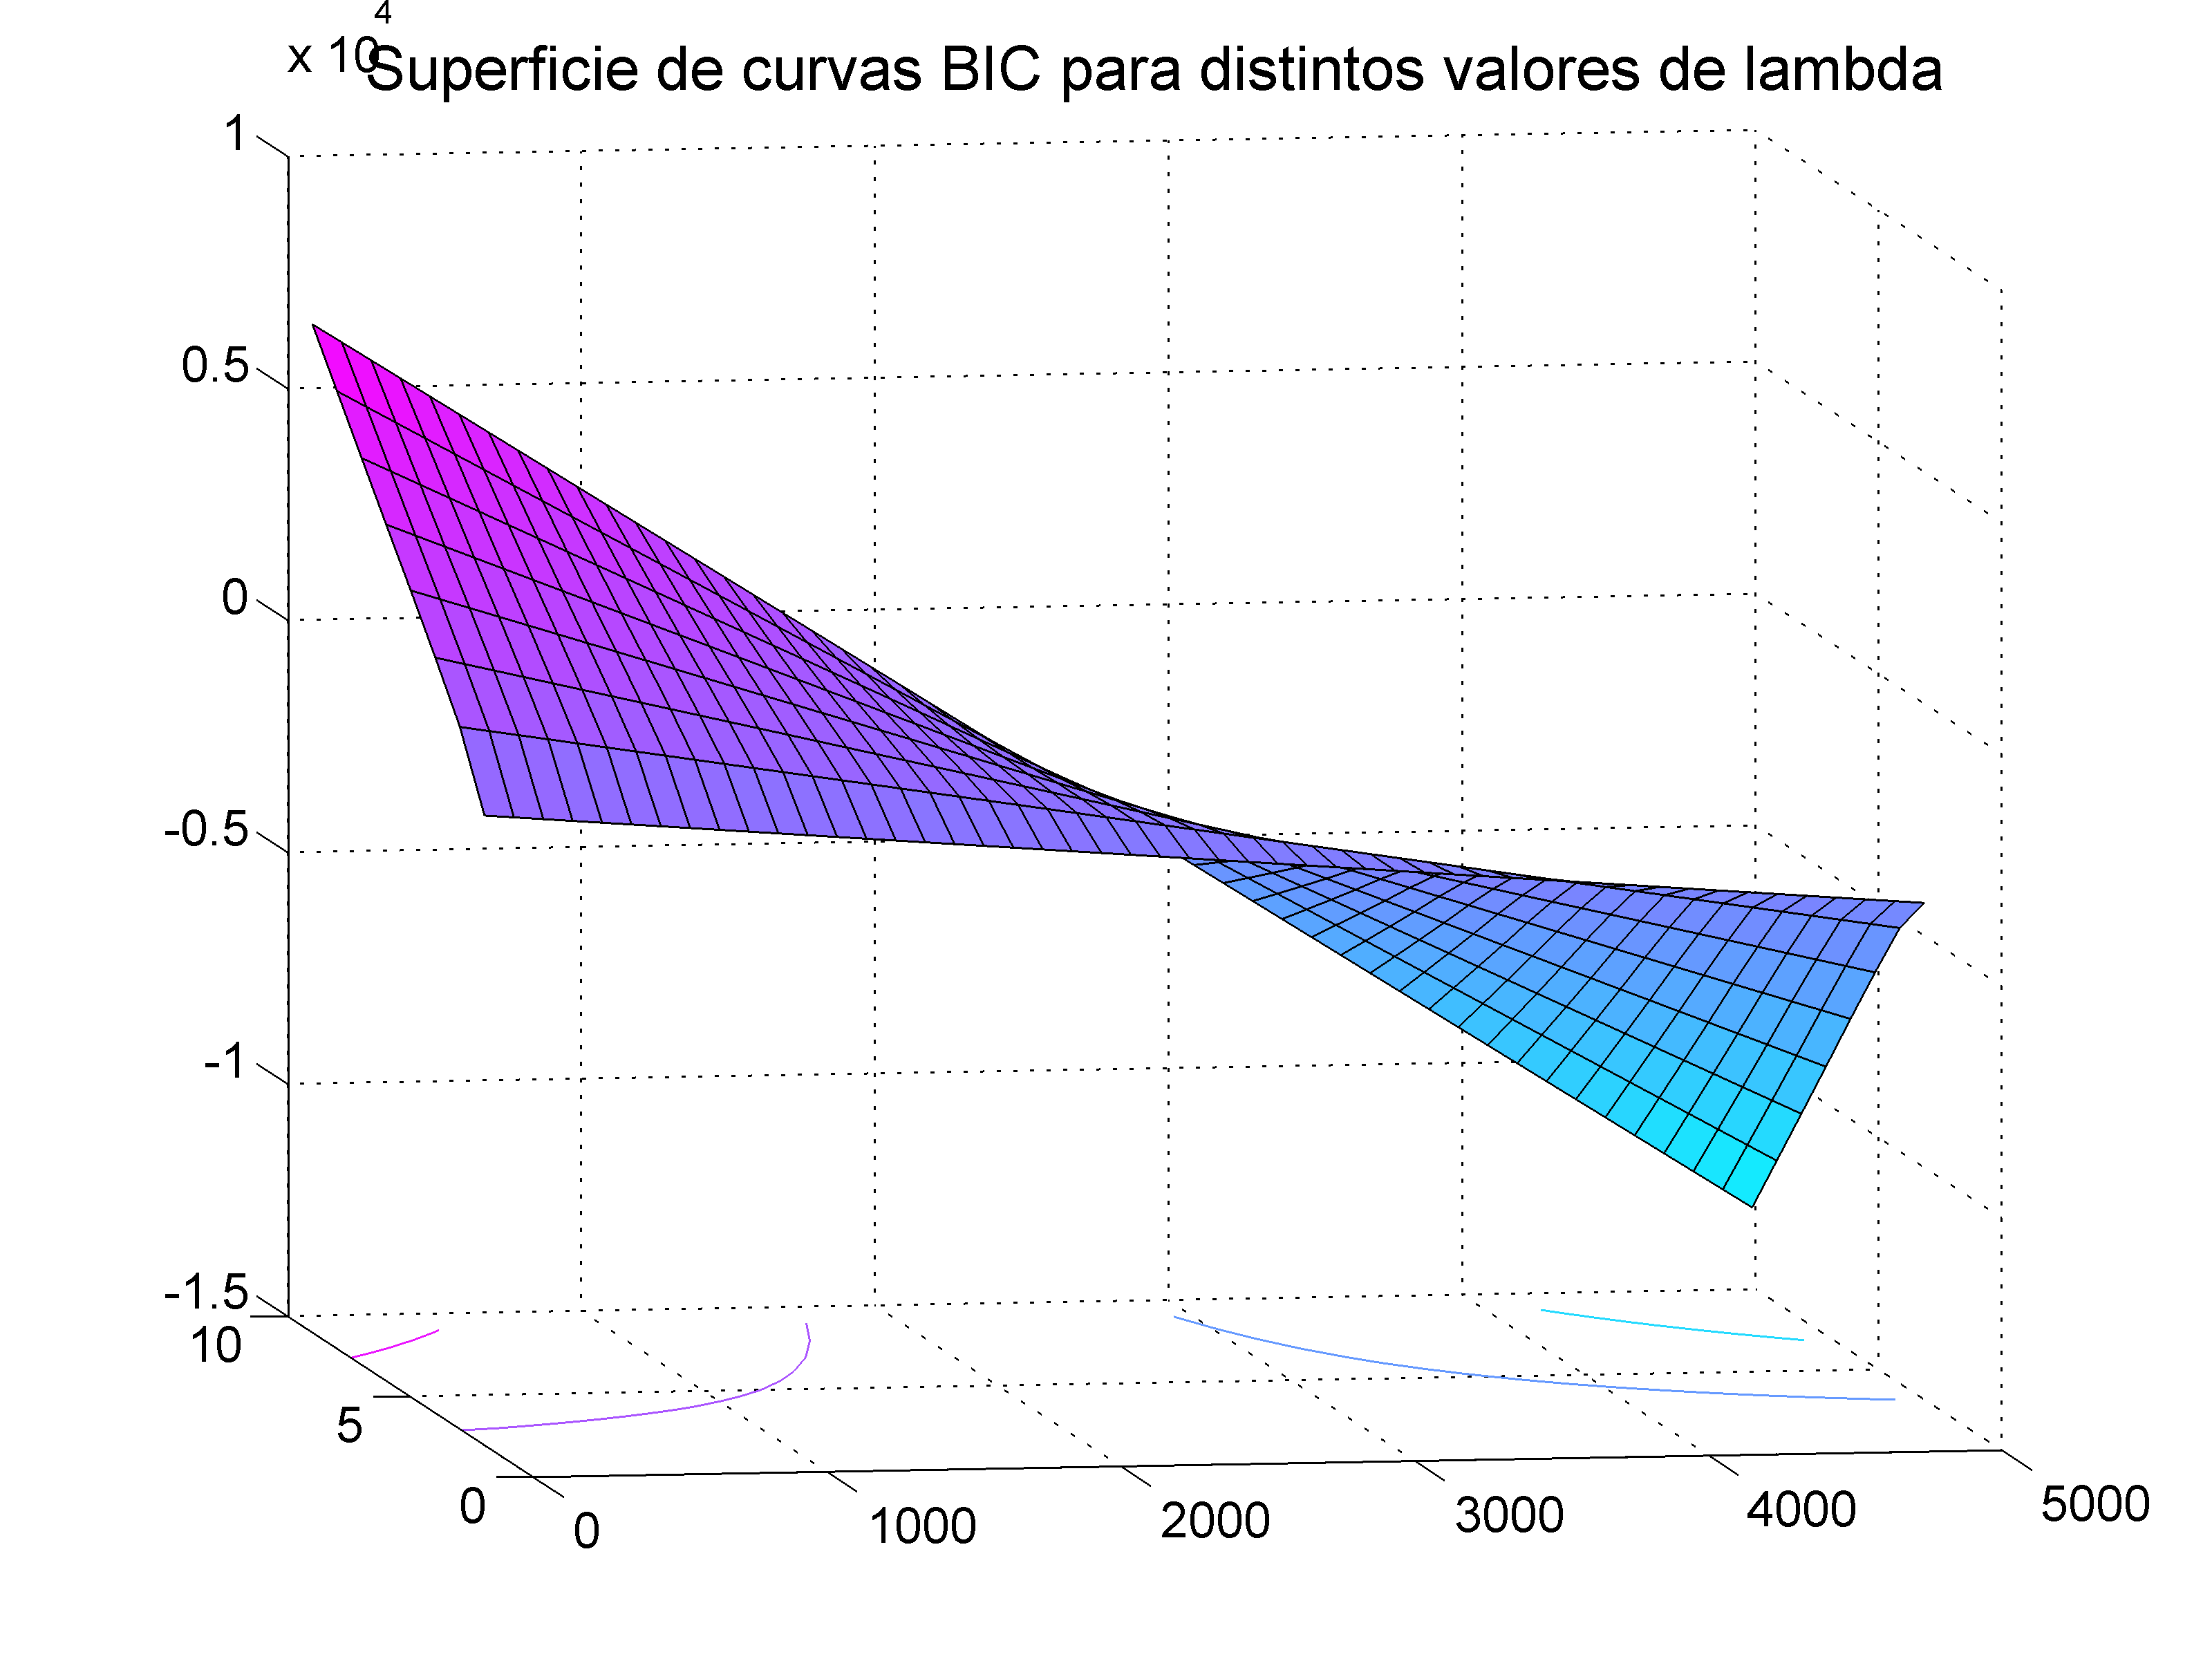
\includegraphics[width=0.8\linewidth]{gfx/chap6/cald20}
   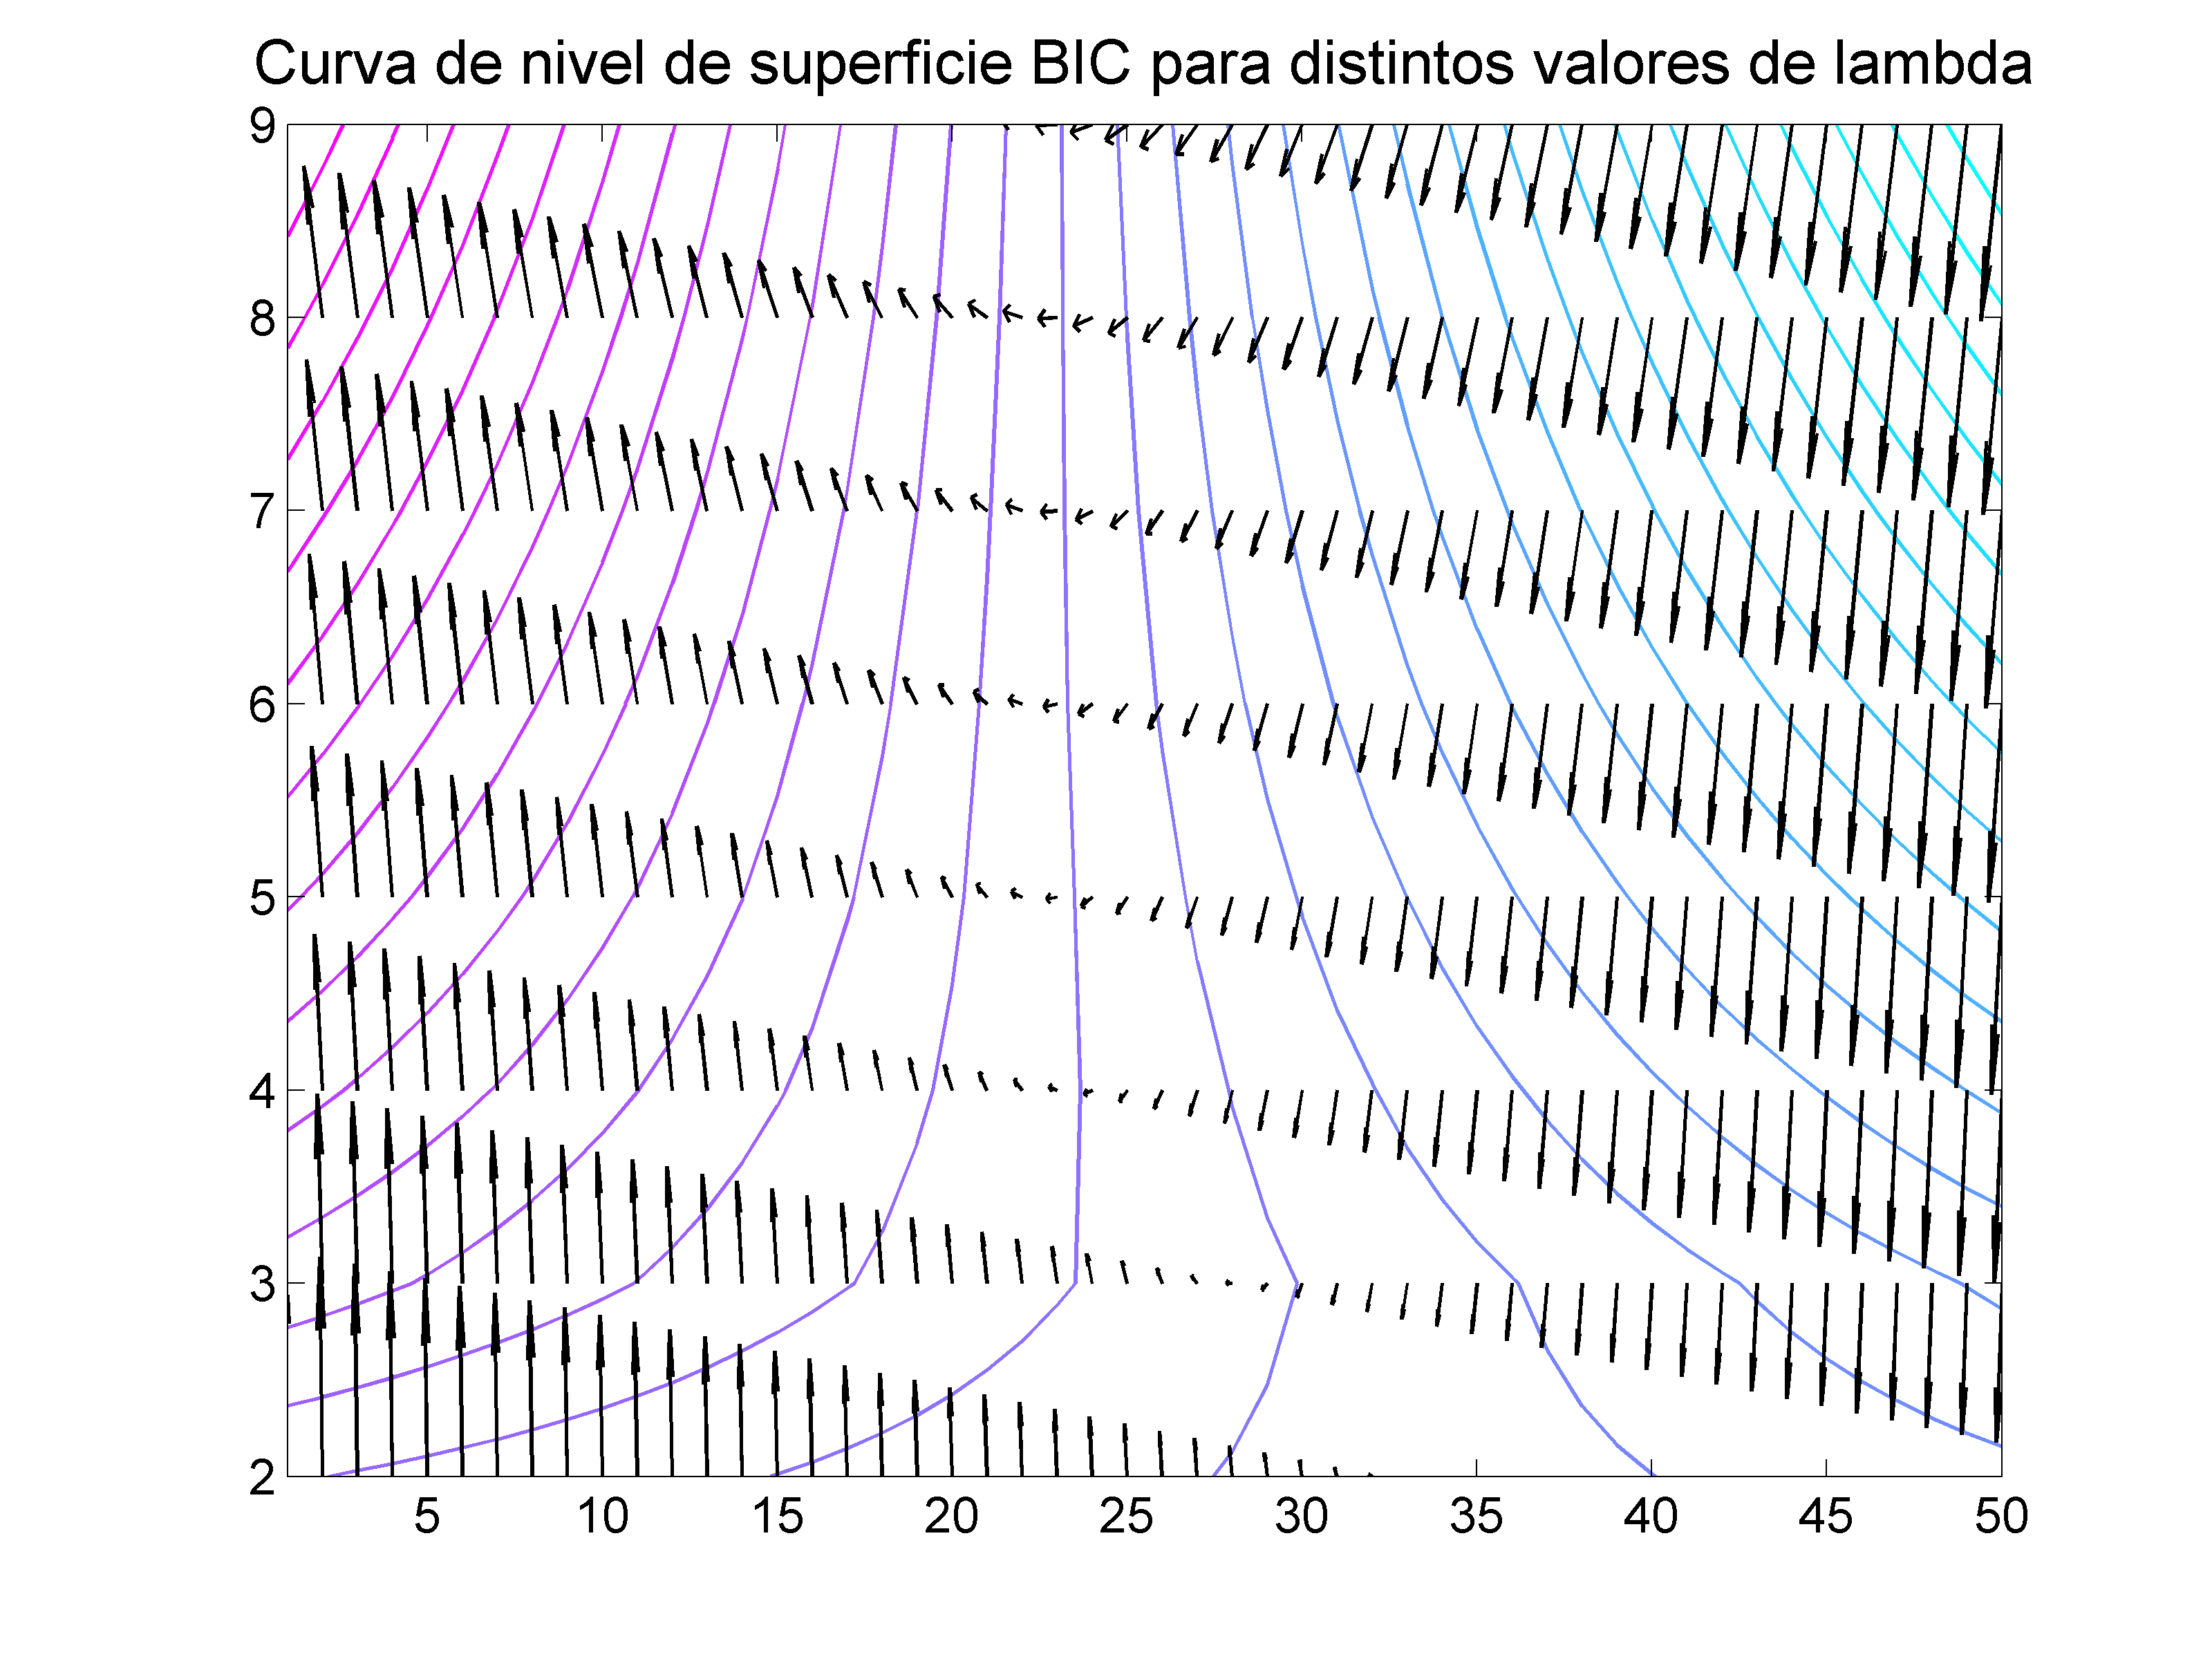
\includegraphics[width=0.8\linewidth]{gfx/chap6/cald21}
  } \quad
  \caption{Superficie y curva de nivel BIC para Prueba 1.}
  \label{fig:prb1_sup}
\end{figure}

\begin{figure}[bth]
  \centerline
  {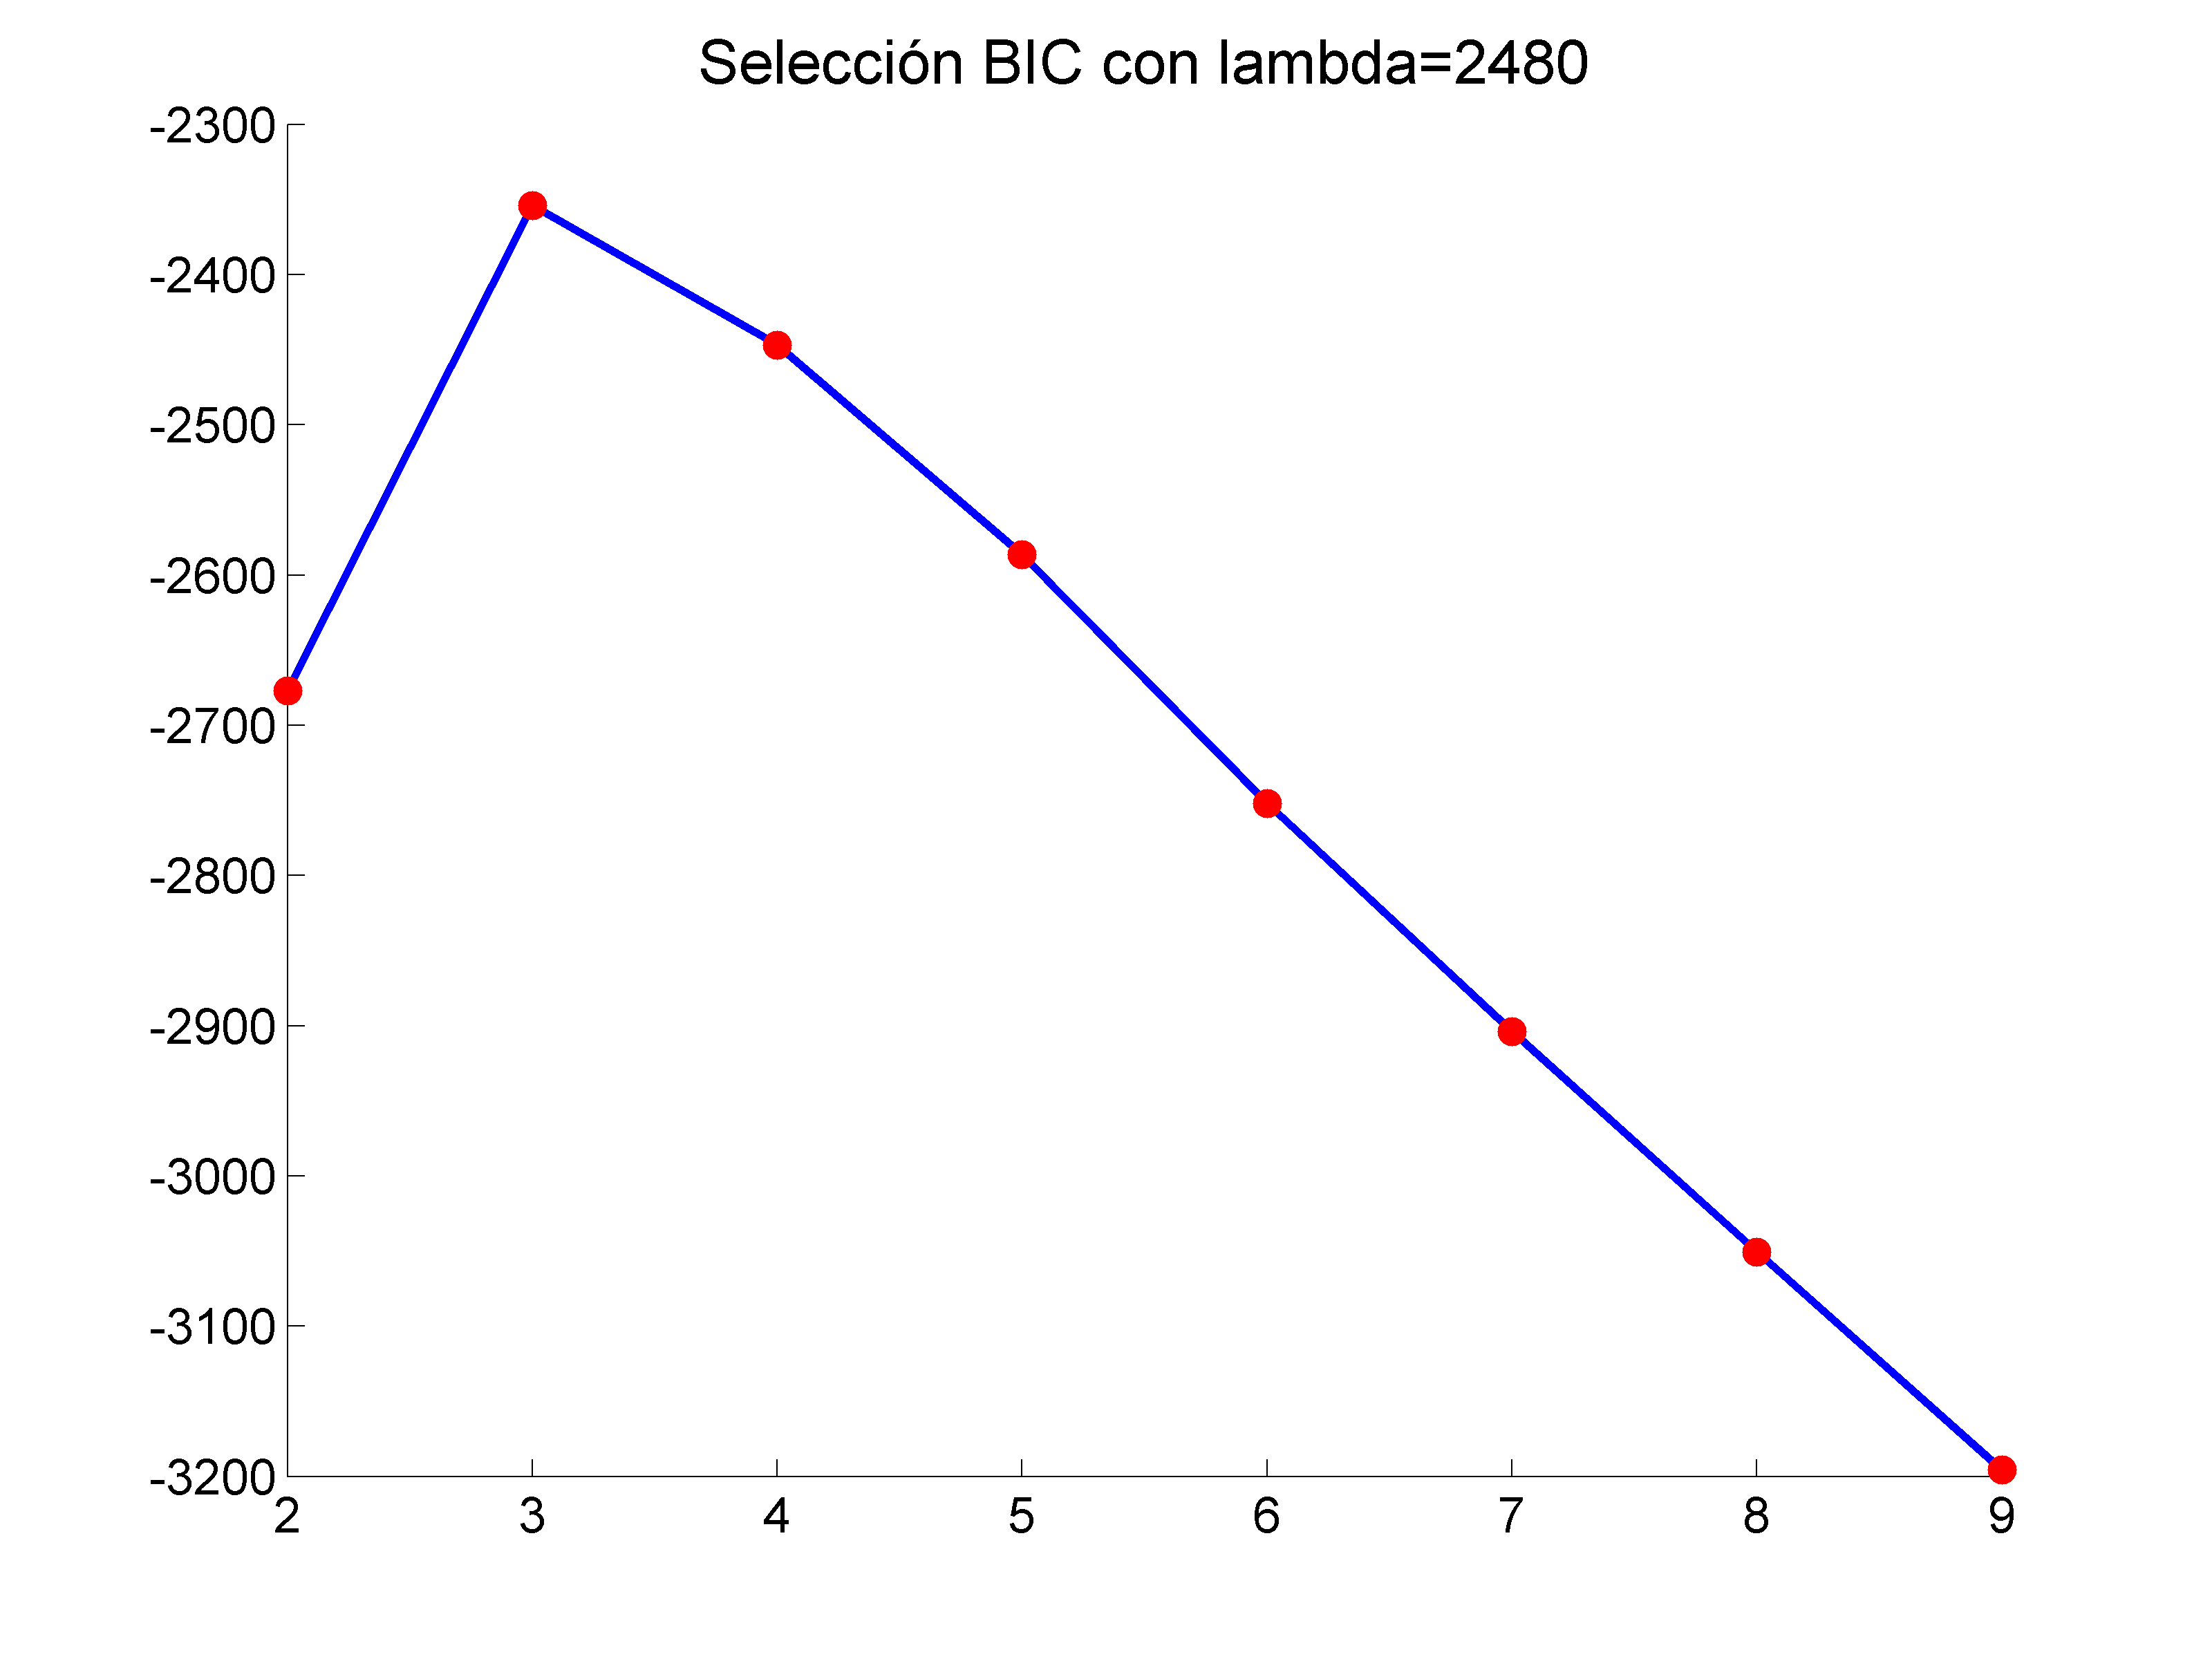
\includegraphics[width=0.8\linewidth]{gfx/chap6/cald11}} \quad
  \caption{Curva BIC con lambda seleccionado para Prueba 1.}
  \label{fig:prb1_curv}
\end{figure}

\begin{figure}[bth]
  \centerline  
  {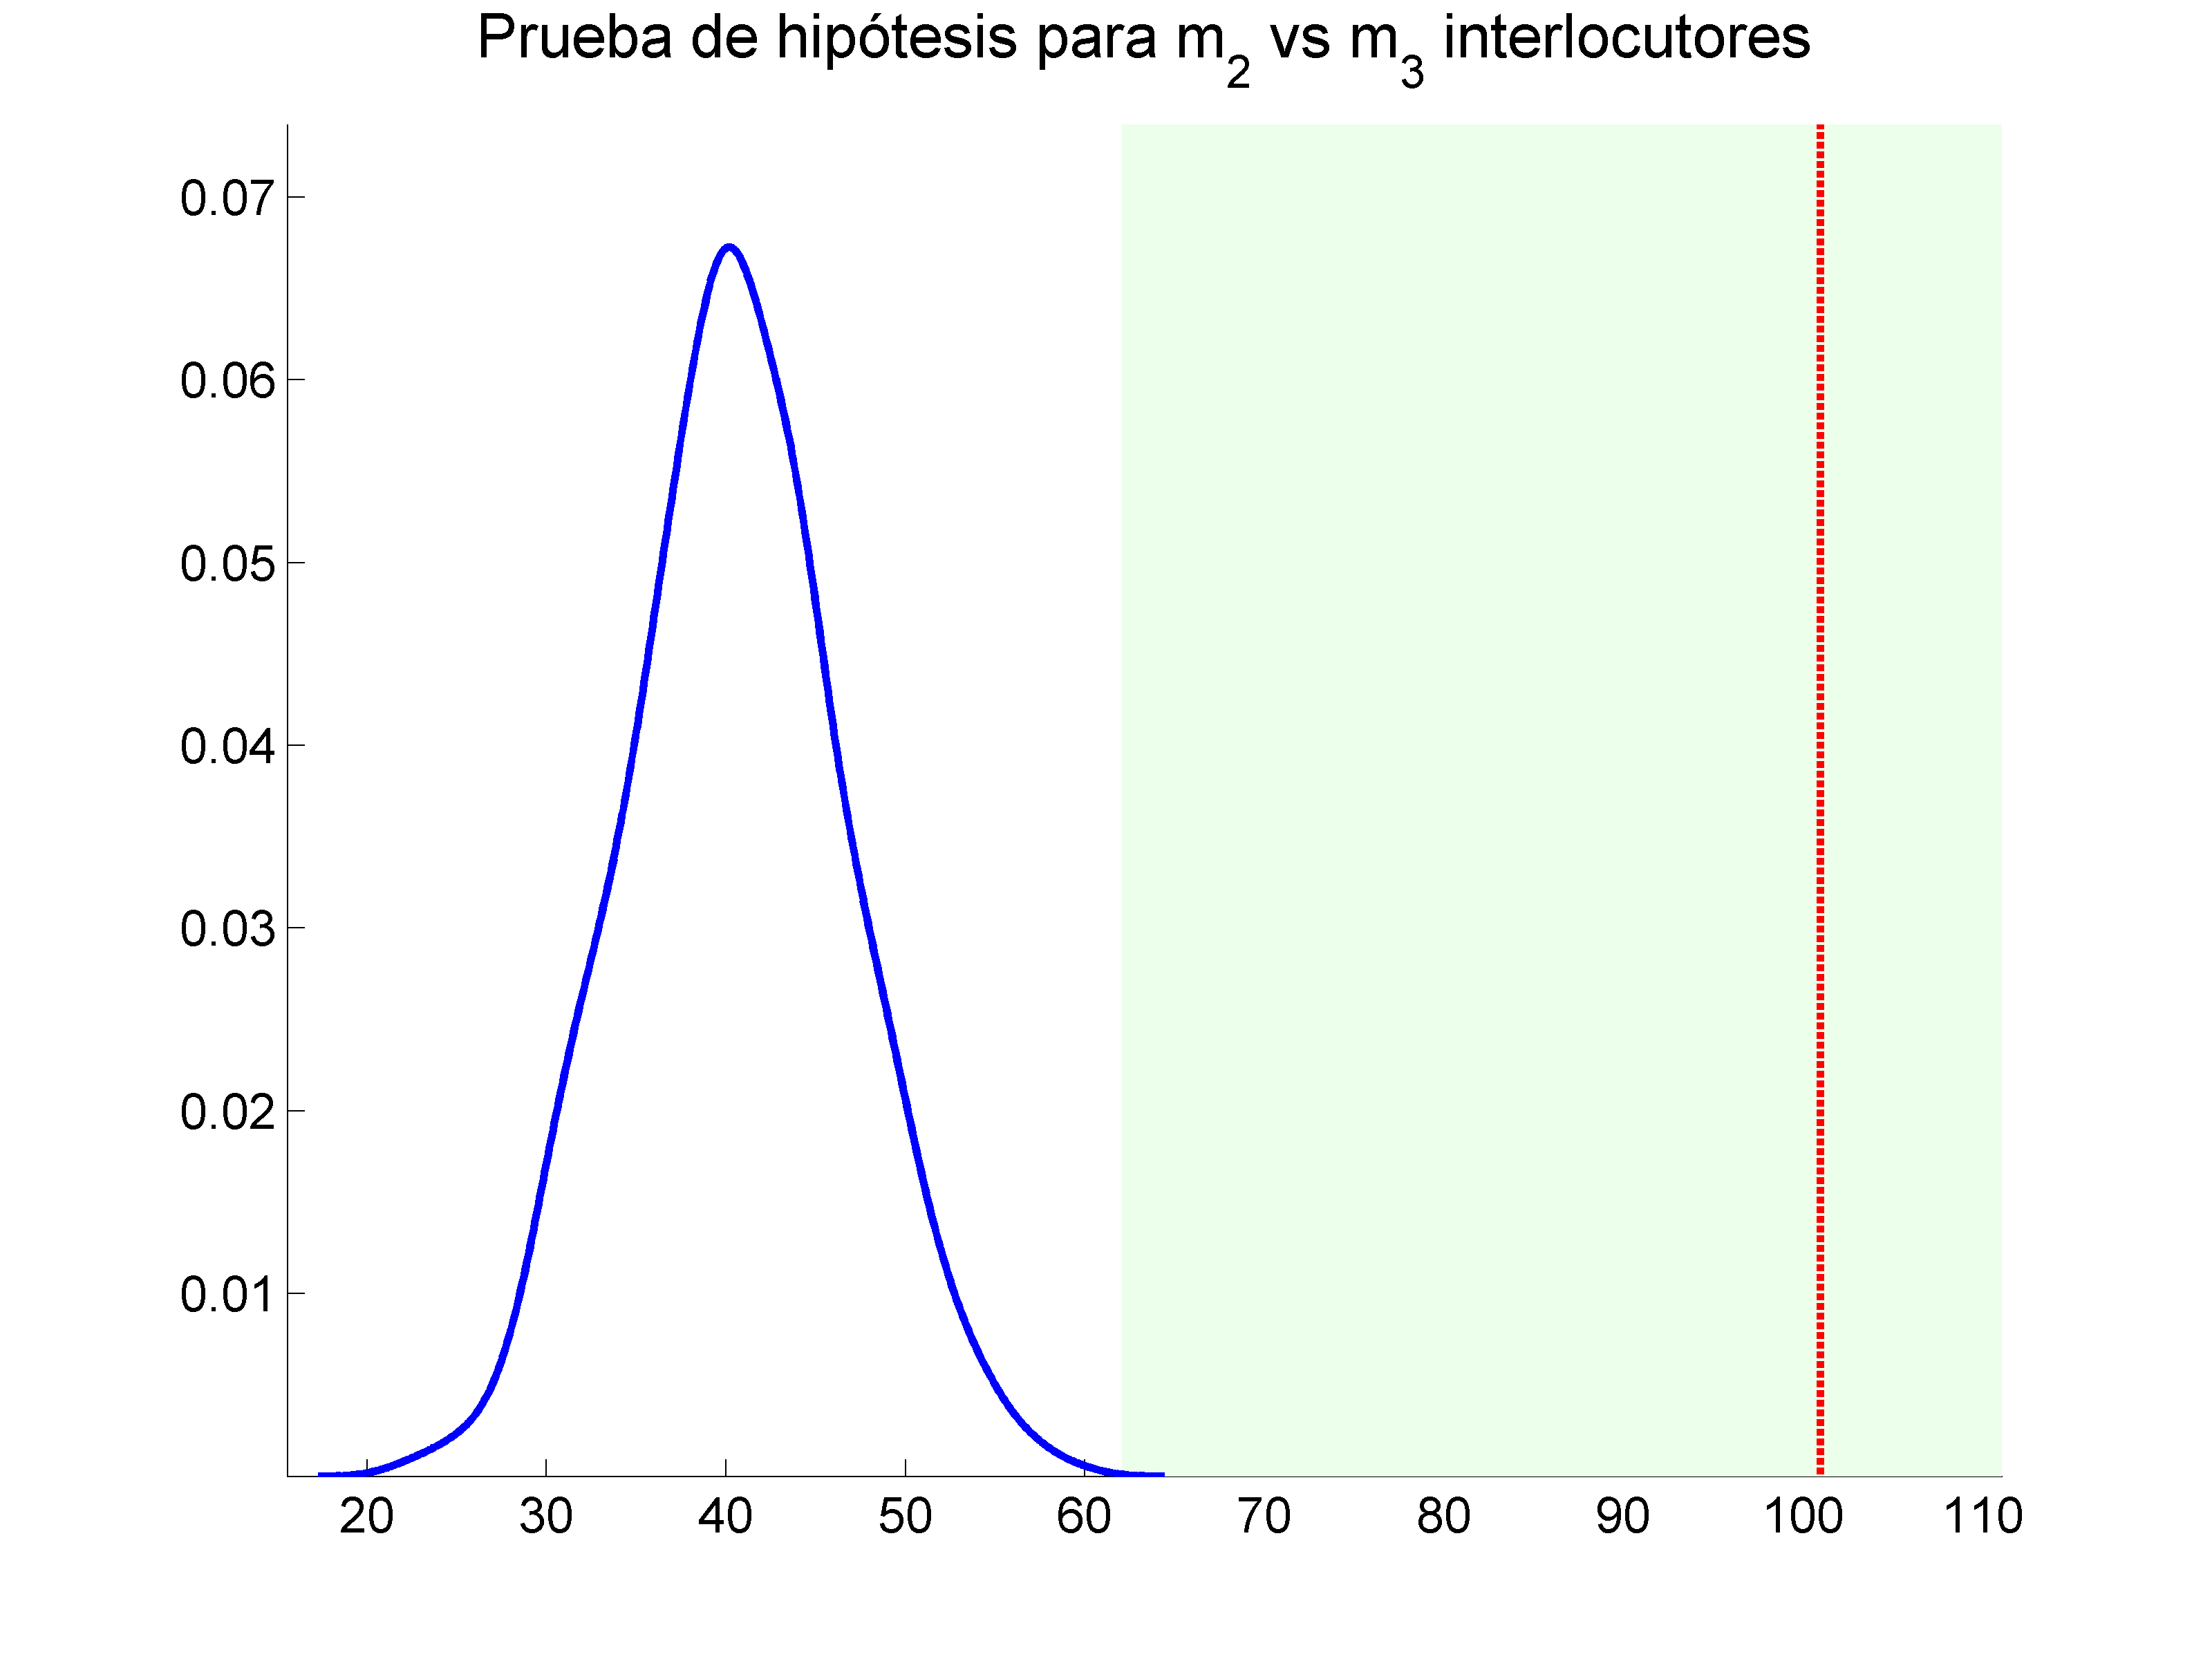
\includegraphics[width=0.8\linewidth]{gfx/chap6/caldb1}
   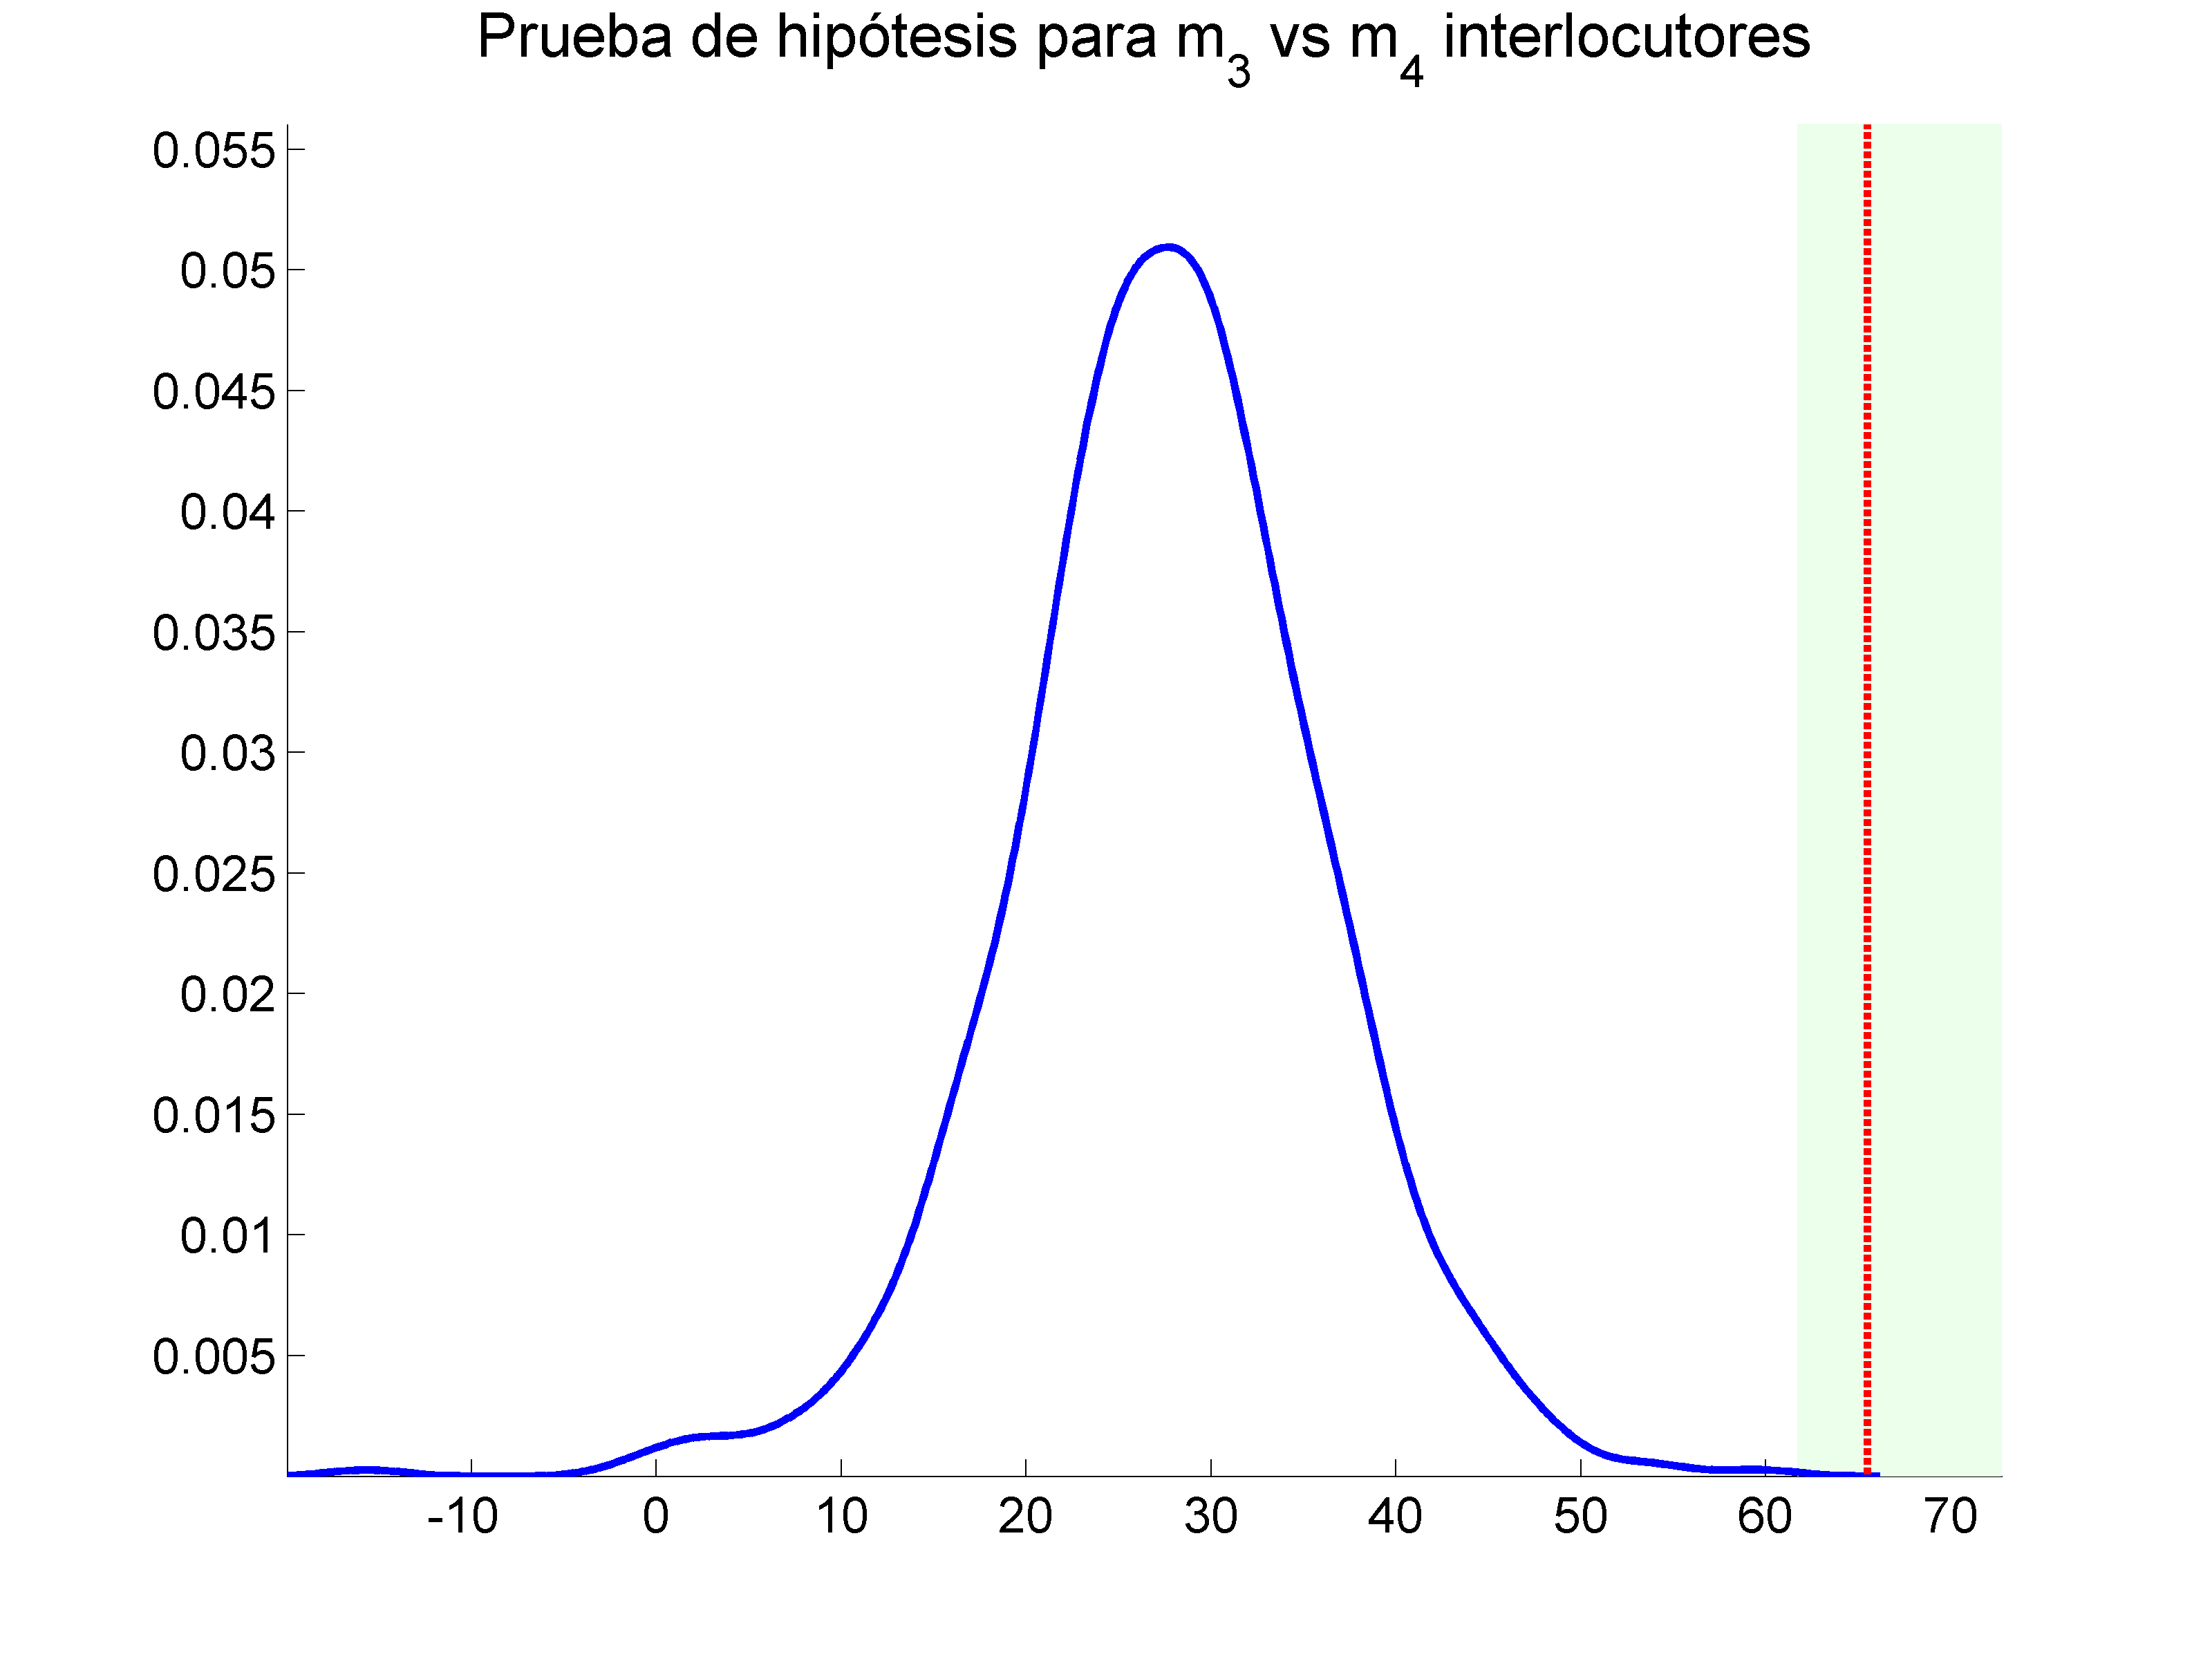
\includegraphics[width=0.8\linewidth]{gfx/chap6/caldb2} }
  \centerline  
  {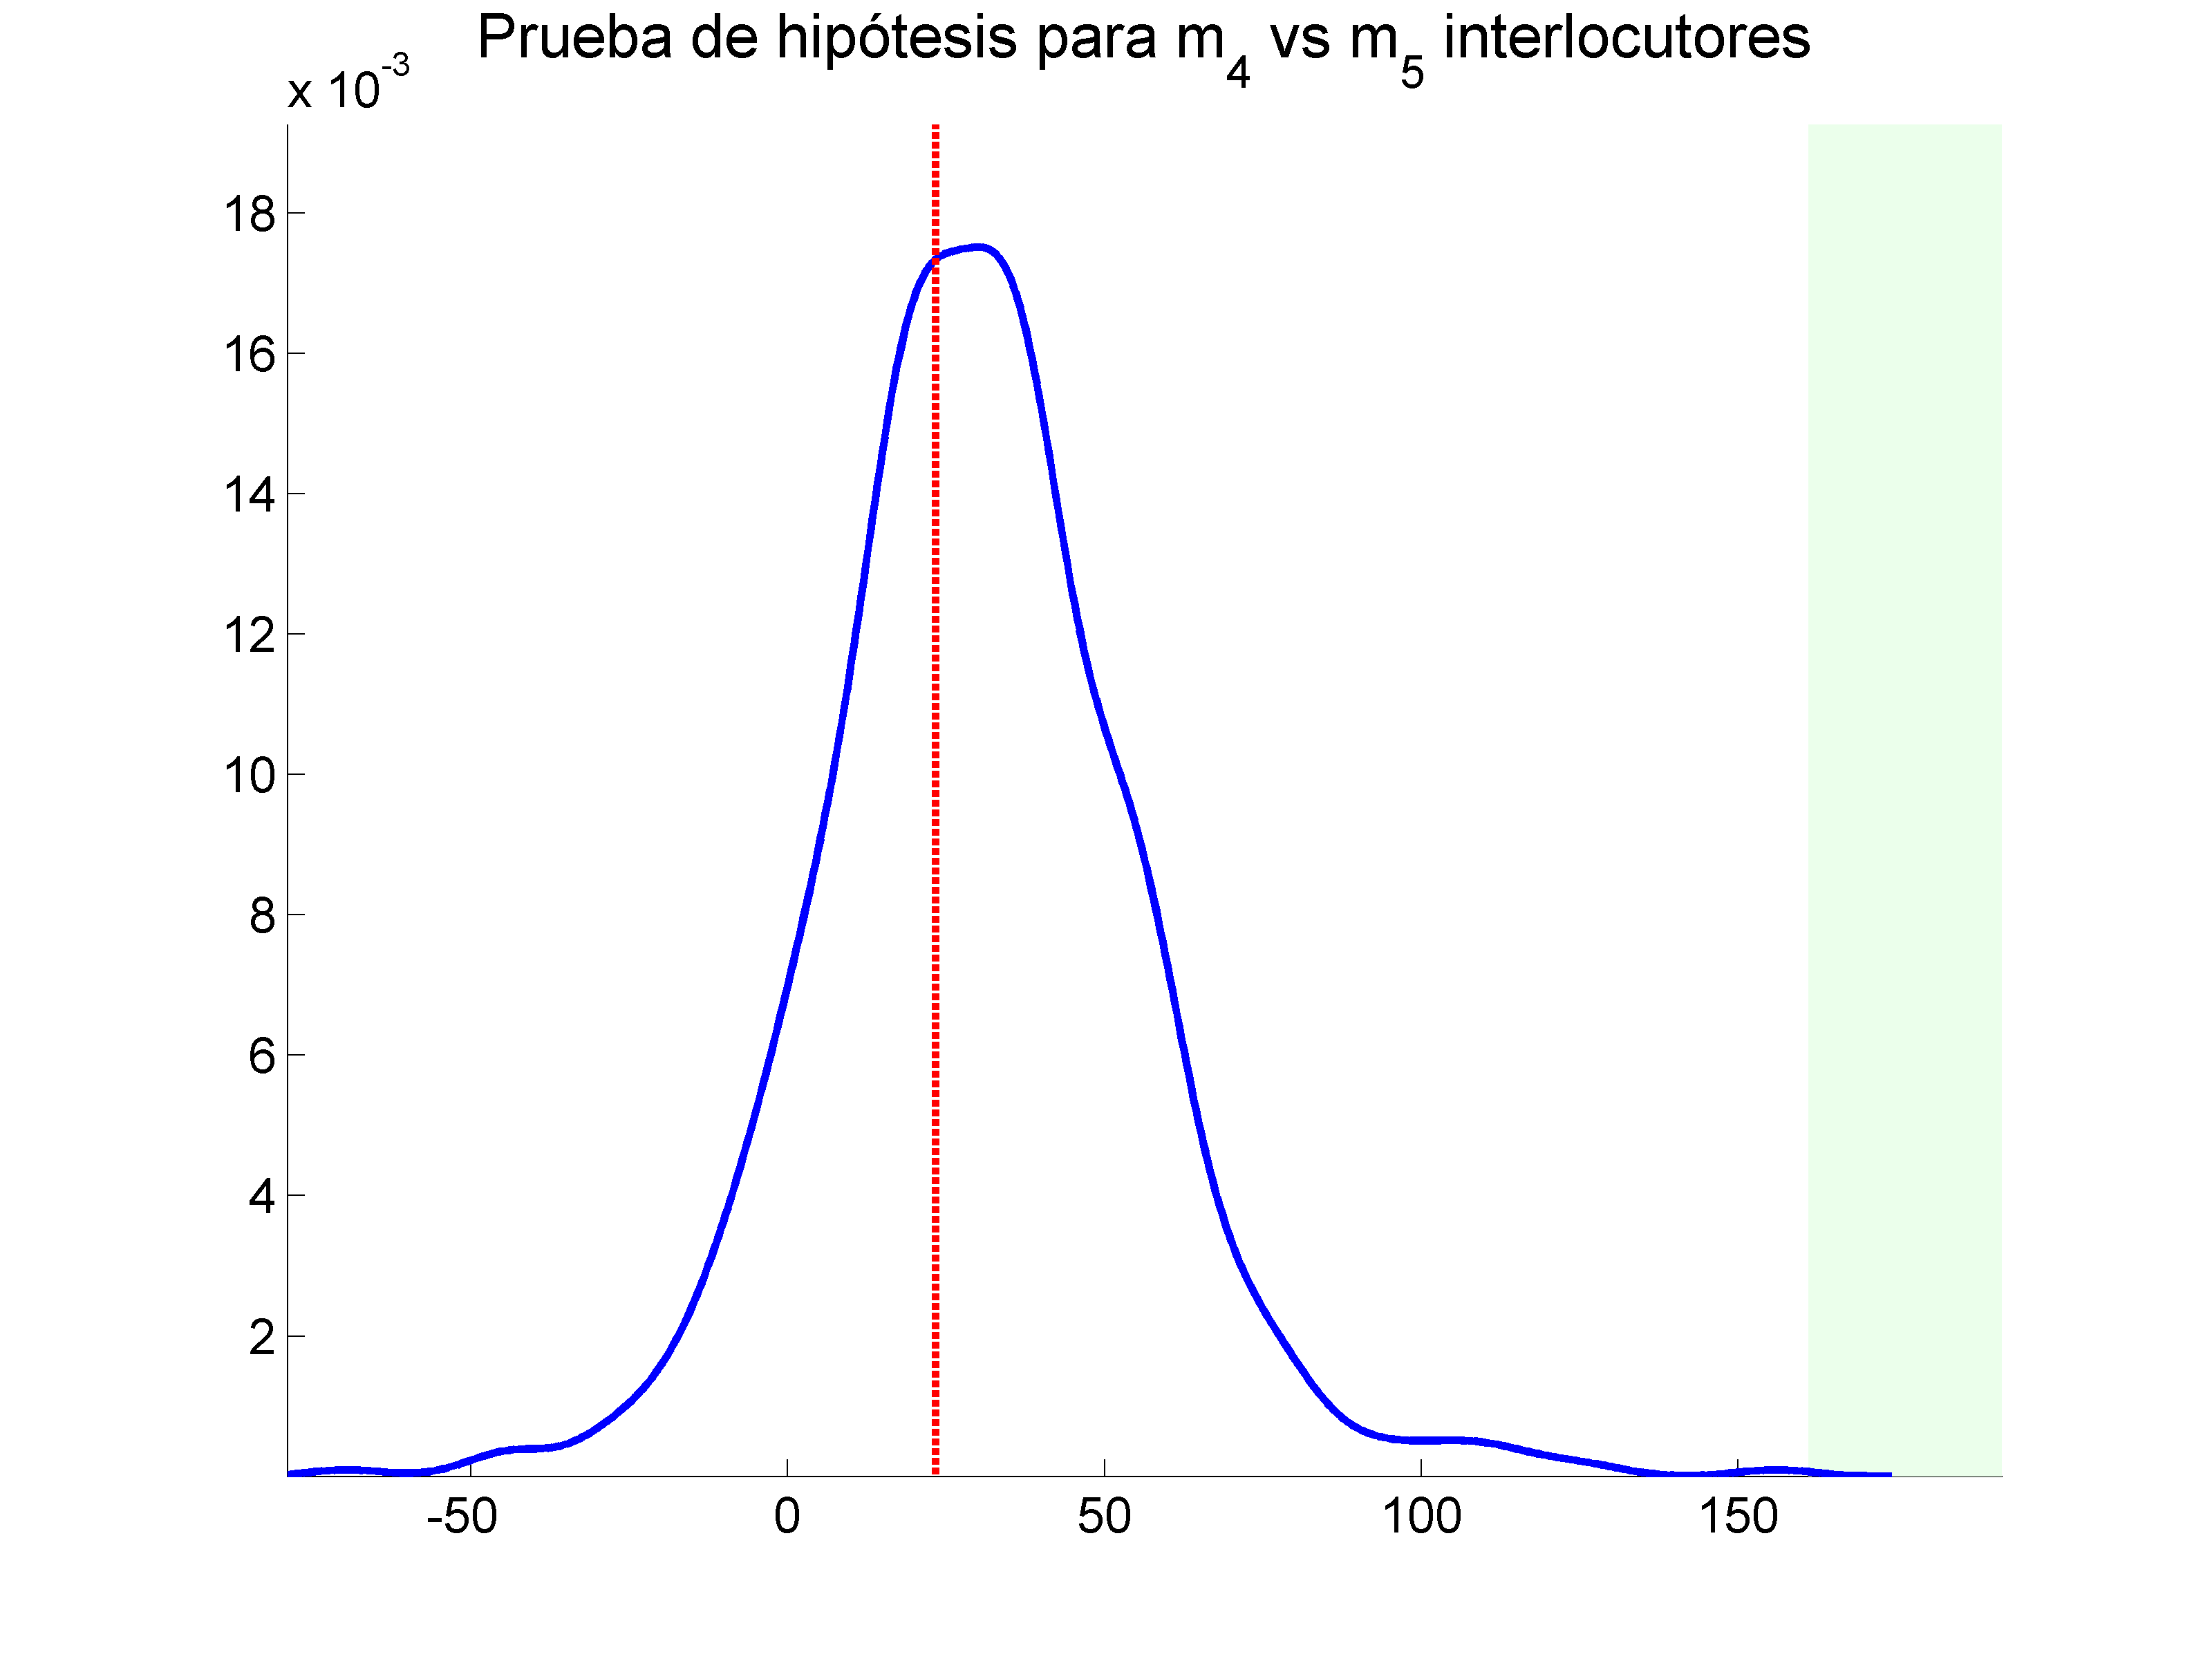
\includegraphics[width=0.8\linewidth]{gfx/chap6/caldb3}
  } \quad
  \caption{Pruebas de hipótesis con bootstrap para Prueba 1.}
  \label{fig:prb1_boot}
\end{figure}

% subsubsection calderon_de_la_barca (end)
% section experimentos (end)